\newpage
\section{Manuel utilisateur}
\label{sec:manuel}


\subsection{En ligne de commande}
\paragraph{} Pour tester nos méthode sans interface on clique sur "run" dans la classe Evenement qui va appeler toutes les classes necessaires a la simulation, l'achat et la vente d'action.
\paragraph{Dans un premier temps on aura l'affichage des informations sur les entreprises.}

%\begin{figure}
%\centering
%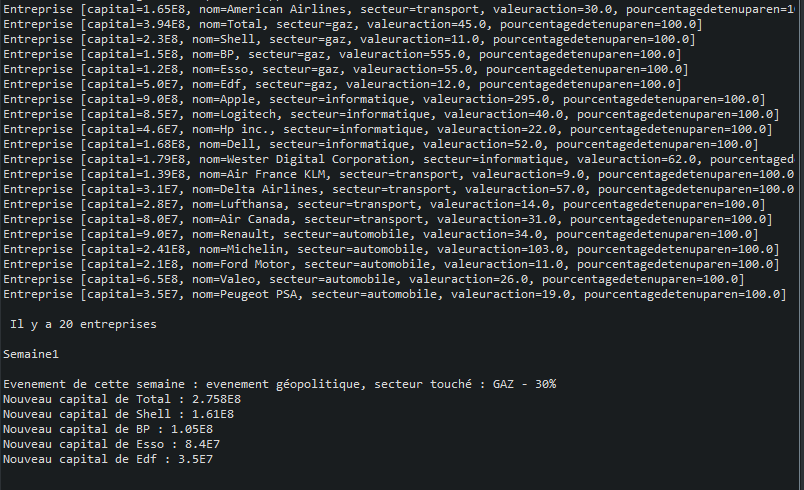
\includegraphics[width=3.5cm, height=2cm]{images/affichage1.png}
%\caption{Affichage CLI}
%\label{fig:modele}
%\end{figure}

\fig{images/affichage1.png}{12cm}{8cm}{Affichage CLI}{Affichage CLI}

\paragraph{]Ensuite on a le choix de faire un ou plusieurs achats/ventes, puis une nouvelle semaine commence.}

%\begin{figure}
%\centering
%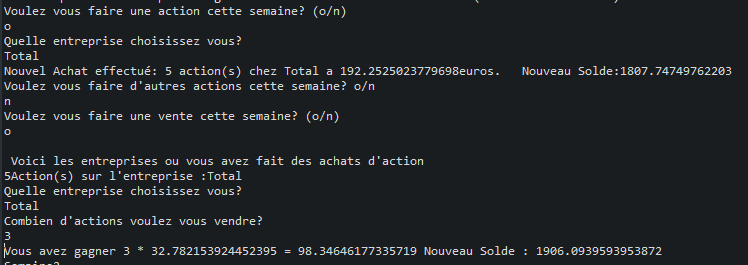
\includegraphics[width=3.5cm, height=2cm]{images/affichage2.png}
%\caption{Affichage CLI2}
%\label{fig:modele}
%\end{figure}

\fig{images/affichage2.png}{12cm}{4cm}{Affichage CLI2}{Affichage CLI2}

\paragraph{}
\paragraph{}
\paragraph{}
\paragraph{}

\subsection{En Interface graphique:}

\paragraph{}En interface graphique on a utilisé la librairie JFreeChart il faut donc installer les 2 fichiers jar jcommon-1.x.jar et jfreechart-1.x.jar telechargeable ici : \url{https://sourceforge.net/projects/jfreechart/} . Il faut ensuite placer les fichier dans un dossier lib dans le dossier source du projet.

\paragraph{}Ensuite dans eclipse il faut clic droit sur le dossier du projet, puis proprietés, Java build Path, librairies, cliquer sur classPath puis add Jar et aller dans le dossier lib pour choisir Jcommon, puis recommencer l'opération avec JFreechart.jar. 

%\begin{figure}
%\centering
%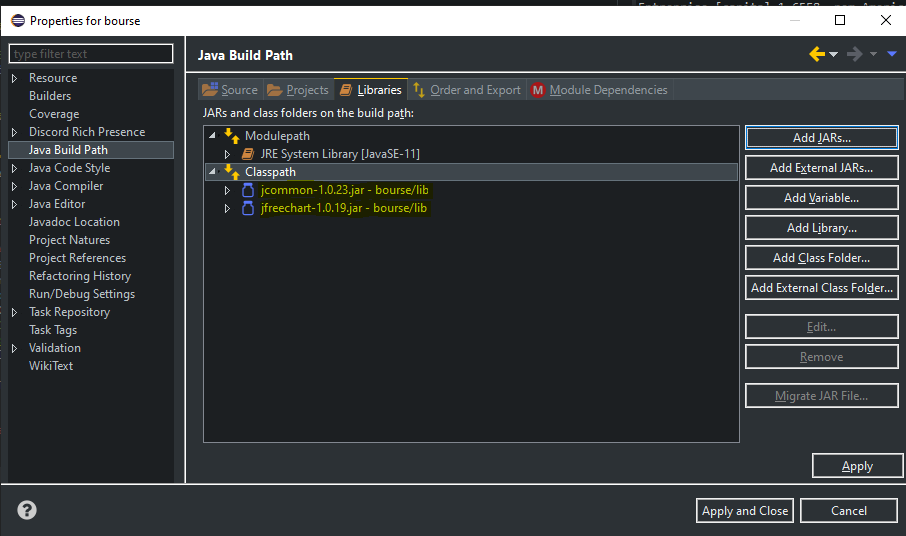
\includegraphics[width=3.5cm, height=2cm]{images/JFreechart.png}
%\caption{JFreechart}
%\label{fig:modele}
%\end{figure}

\fig{images/JFreechart.png}{13cm}{8.5cm}{JFreechart}{JFreechart}

\paragraph{}Ensuite on redemarre Eclipse.

\paragraph{} Pour lancer l'interface graphique, on clique sur "run" dans la classe GUI.

\paragraph{} On peut passer de la première a la deuxième fenêtre en cliquant sur le bouton haut de la fenêtre.

\paragraph{} Pour les fonctionnalités de l'interface elles sont assez simples a comprendre, on a juste a cliquer sur l'entreprise qu'on veut puis cliquer sur "choisir" pour l'afficher sur le graphique (cliquer sur la zone blanche du graphique si il ne s'affiche pas).
\paragraph{} En cliquant sur play une semaine passera et donc la zone news sera mise a jour.
\paragraph{} Sur la deuxième fenêtre pour vendre ou acheter des action on choisit son entreprise puis le nombre d'action et on clique sur "valider".

